\section{MTU Discovery}
\label{sec:MTU Discovery}

\subsection{Einleitung}
todo theo

%TODO: statt Rechner 1 und 2 Alice und Bob verwenden!
\subsection{Idealer Ablauf bei der MTU-Bestimmung}
Dieses Sequenz-Diagramm stellt den idealen Ablauf bei der MTU-Bestimmung dar. Rechner 1 schickt Rechner 2 ein Paket mit dem Kommando 'MTU?'. Dieses Paket hat eine typische Grösse gem. Erfahrungswerten. Momentan starten wir mit 500Bytes. %TODO: CITATION NEEDED! GRÖSSE ANPASSEN
Rechner 2 erhält das Paket und schickt eine Antwort mit dem Kommando 'OK'. Darauf erhöht Rechner 1
die Grösse des Pakets um einen konfigurierbaren Inkrementationswert und schickt es wieder zurück an
Rechner 2. Dieser Ablauf wird so lange wiederholt bis das Paket nicht mehr bei Rechner 2 ankommt.
Weil das Paket nicht ankommt kann Rechner 2 keine Antwort senden und Rechner 1 läuft in ein Timeout.
Rechner 1 nimmt jetzt den letzten erfolgreichen MTU-Wert und schickt Rechner 2 erneut ein Paket.
Wenn das Paket erfolgreich ankommt, d.h. Rechner 2 ein 'OK' zurückschickt wurde die MTU erfolgreich gefunden. Rechner 1 setzt nun einen Meldung ab das die ideal MTU für die Verbindung zwischen Rechner 1 und 2 gefunden wurde.

% GFX Trim left bottom right top
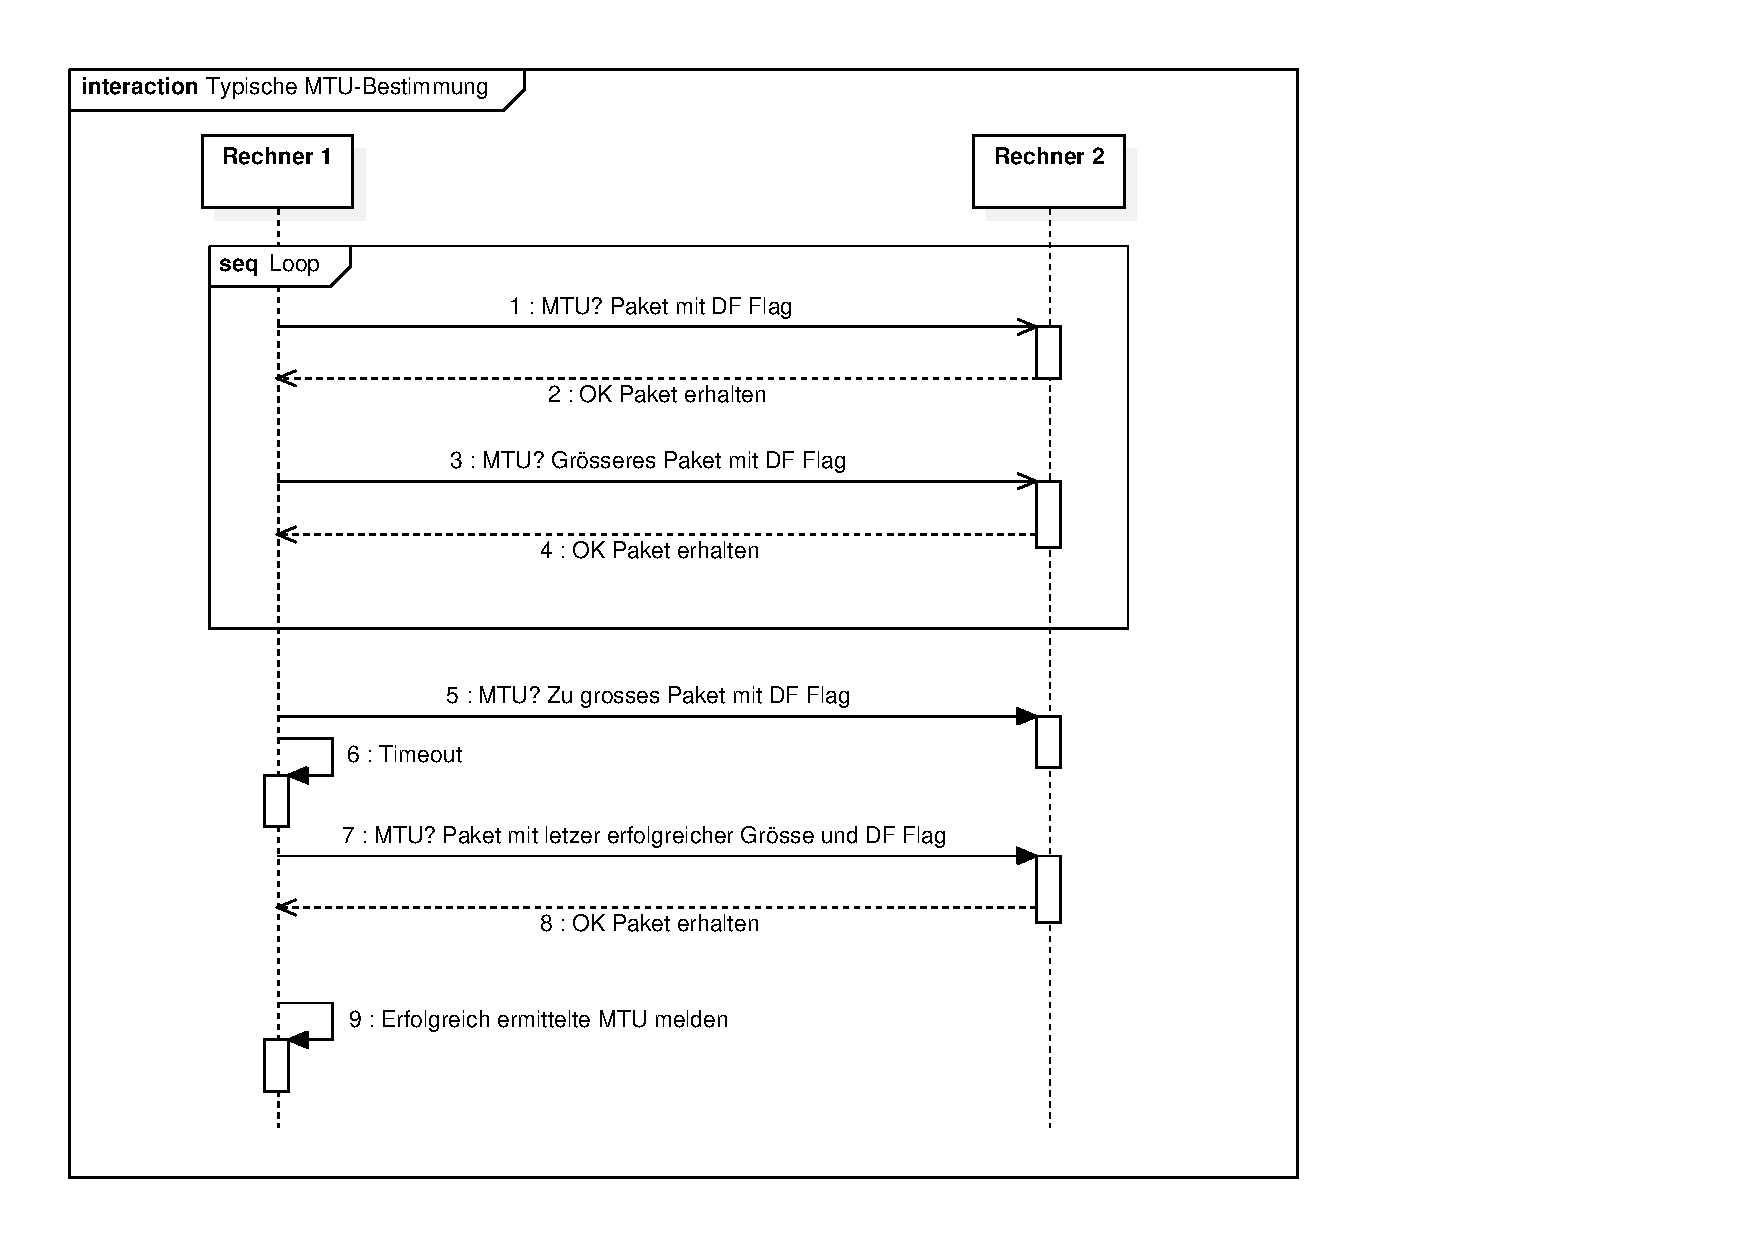
\includegraphics[trim=10 10 200 10,clip,width=\textwidth]{mainpart/implementation/img/typischeMTUBestimmung}